\normaltrue
\correctionfalse

%\UPSTIidClasse{11} % 11 sup, 12 spé
%\newcommand{\UPSTIidClasse}{12}

%\exer{Roue avant de GC10 -- V8 $\star$ \label{A5:05:87}}
\subsection*{Élévateur de Nacelle BEA33}
\setcounter{question}{0}
%\UPSTIcompetence[2]{A5-05}
%\UPSTIcompetence[2]{A5-04}

\index{Compétence A5-05}
\index{Compétence A5-04}

\index{GPS}
\index{Spécification géométrique des produits}

\ifcorrection
\else
\marginnote{\textbf{Pas de corrigé pour cet exercice.}}
\fi


\ifprof
\else
\fi


On s'intéresse à la << palette d'horizontalité >> d'un élévateur de nacelle. 

\begin{center}
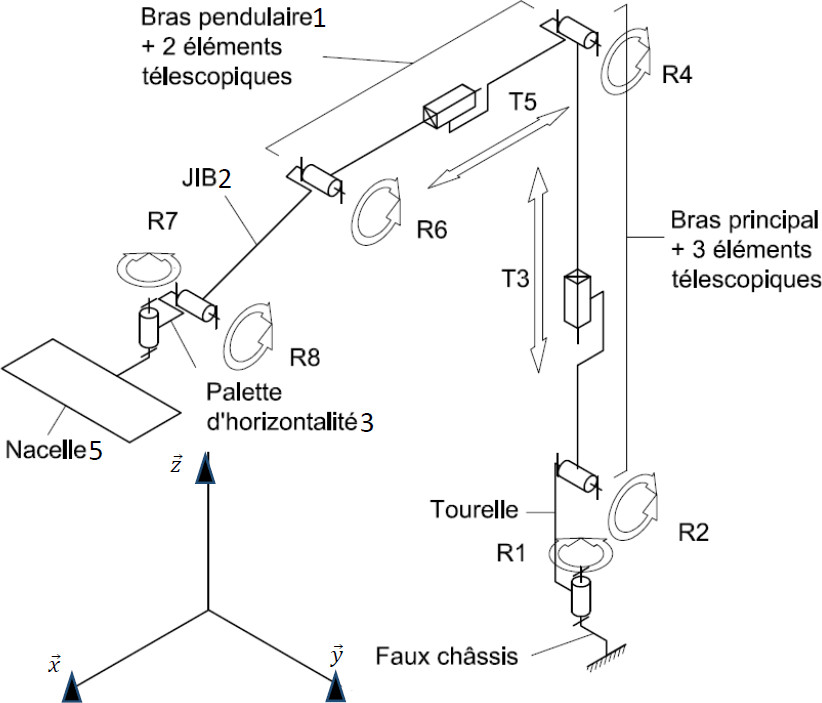
\includegraphics[height=5cm]{87_fig_01}
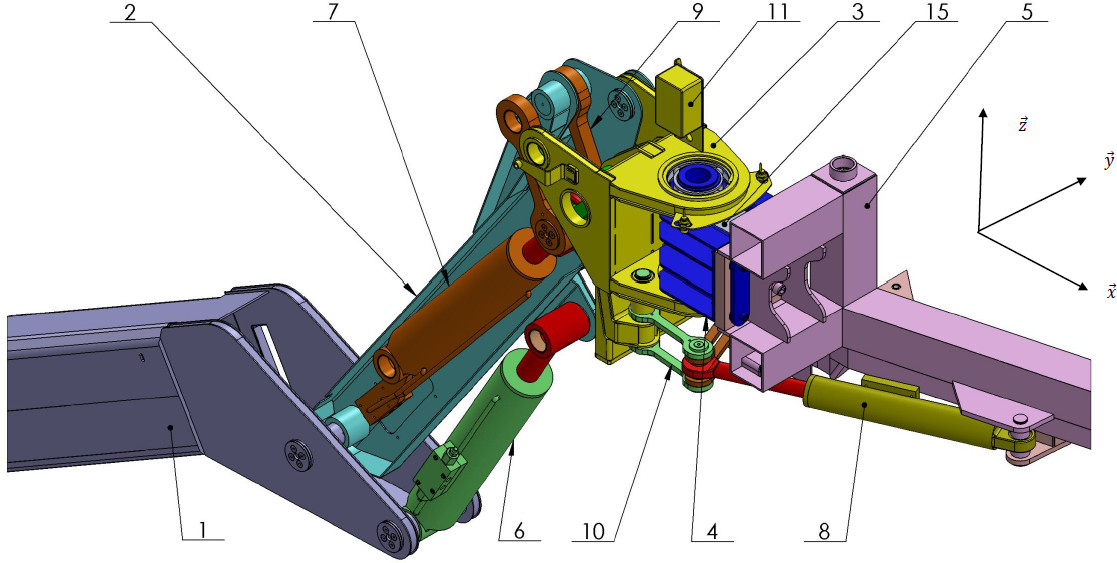
\includegraphics[height=5cm]{87_fig_02}
\end{center}

Une des rotations de la nacelle est assurée par la palette \textbf{3}.
Le plan d'ensemble au verso montre l'assemblage de la palette avec les autres constituants. 

\subsection*{Analyse des spécifications géométriques et dimensionnelles}
\marginnote{On a : $\phi 150 K7 = 150^{\begin{array}{c} +12 \\ -28 \end{array}}$.}

\question{Expliquer quelle(s) fonction(s) du produit justifie l'existence des spécifications suivantes :

\includegraphics[height=.6cm]{87_gps_01} et 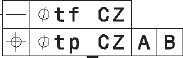
\includegraphics[height=.6cm]{87_gps_02}.}


\question{Décrire les spécifications suivantes :

\includegraphics[height=.6cm]{87_gps_01}, 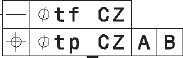
\includegraphics[height=.6cm]{87_gps_02} et  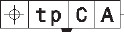
\includegraphics[height=.6cm]{87_gps_03}.}

\question{Partant de la première sépcification de localisation, quelle serait l'influence d'un modificateur au maximum de matière sur l'intervalle de tolérance  ? sur l'élément de référence ? }


\subsection*{Analyse des procédés de fabrication}
\question{Donner l'ensemble des moyens de fabrications ayant mené à la réalisation de la palette.}

\question{Proposer une gamme d'usinage permettant la réalisation de la palette.}

%\end{multicols}



%\begin{center}
%\rotatebox{270}{\includegraphic[height=\linewidth]{87_fig_04}}
%\rotatebox{270}{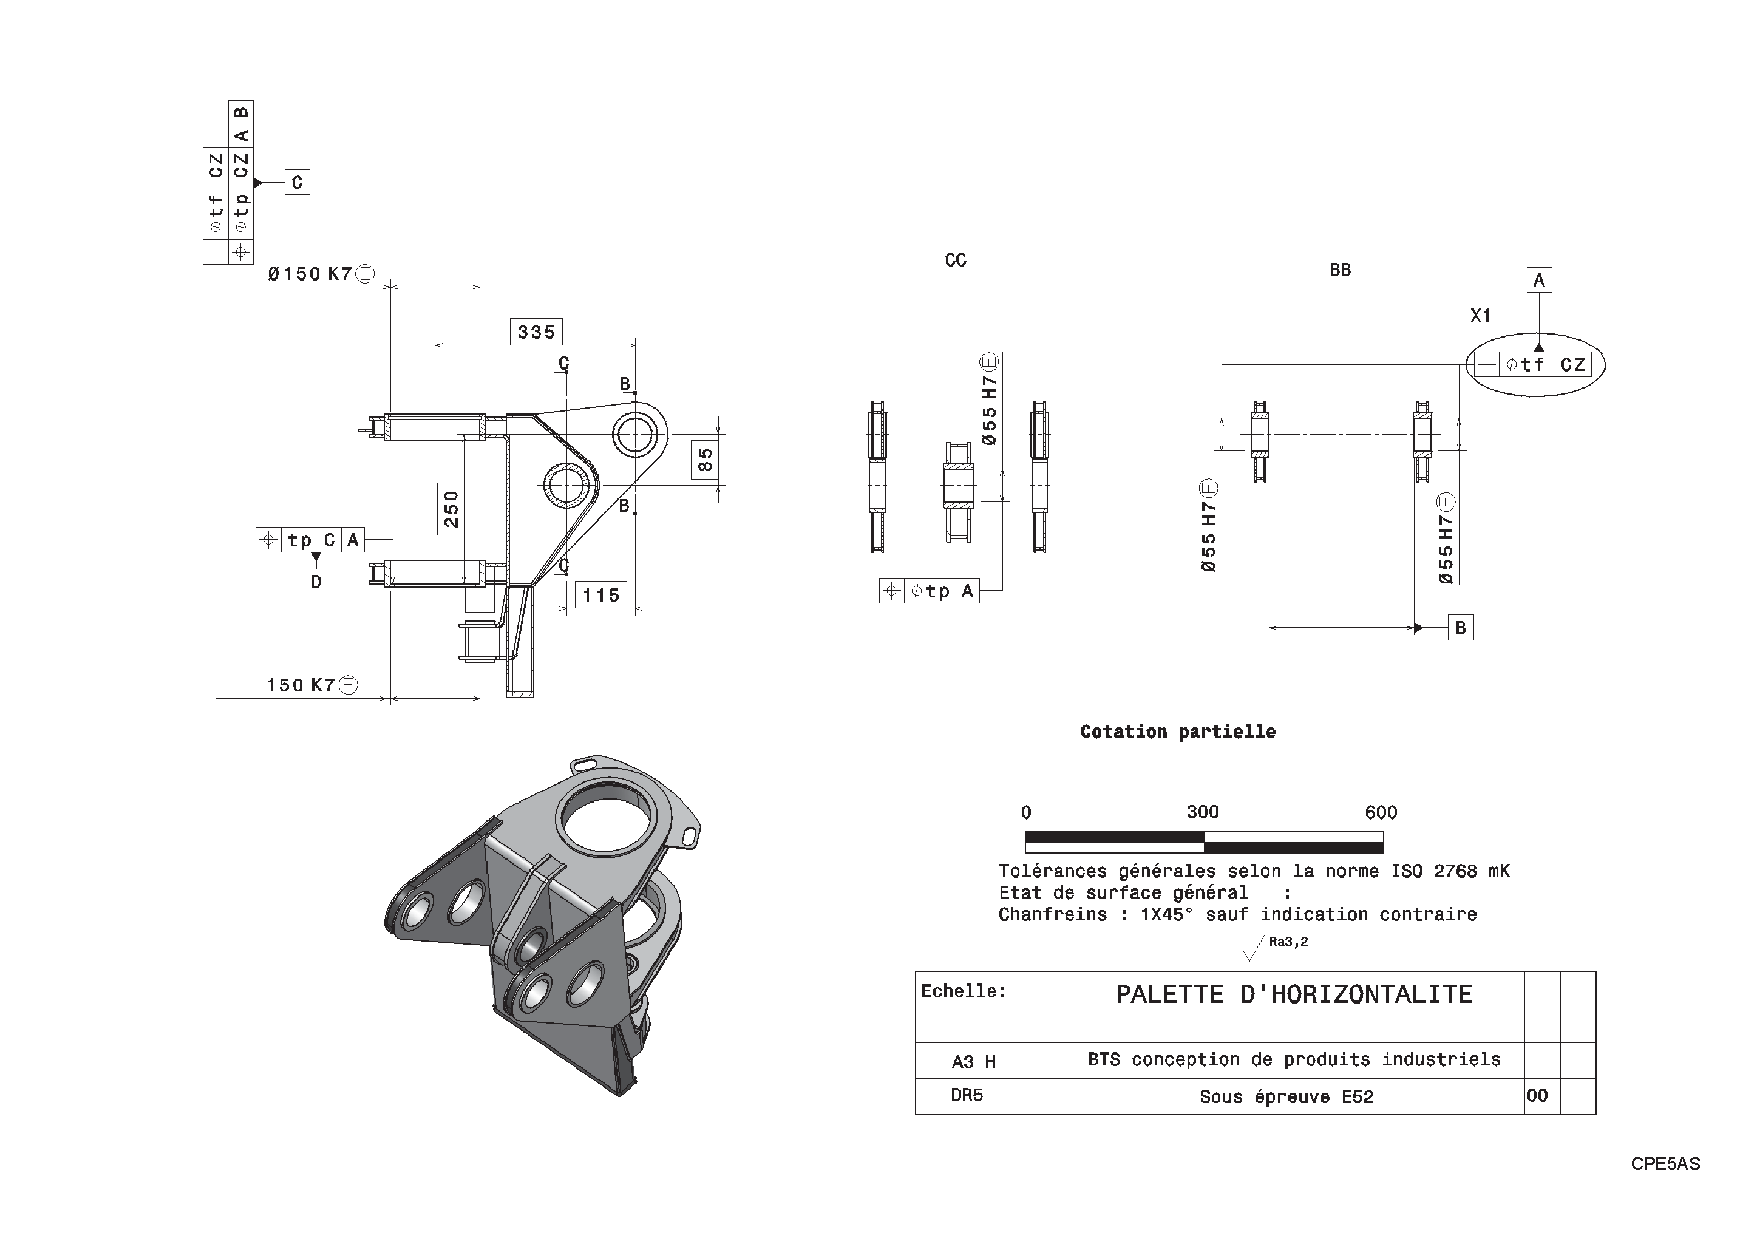
\includegraphics[height=\linewidth]{87_plan_02}}
%{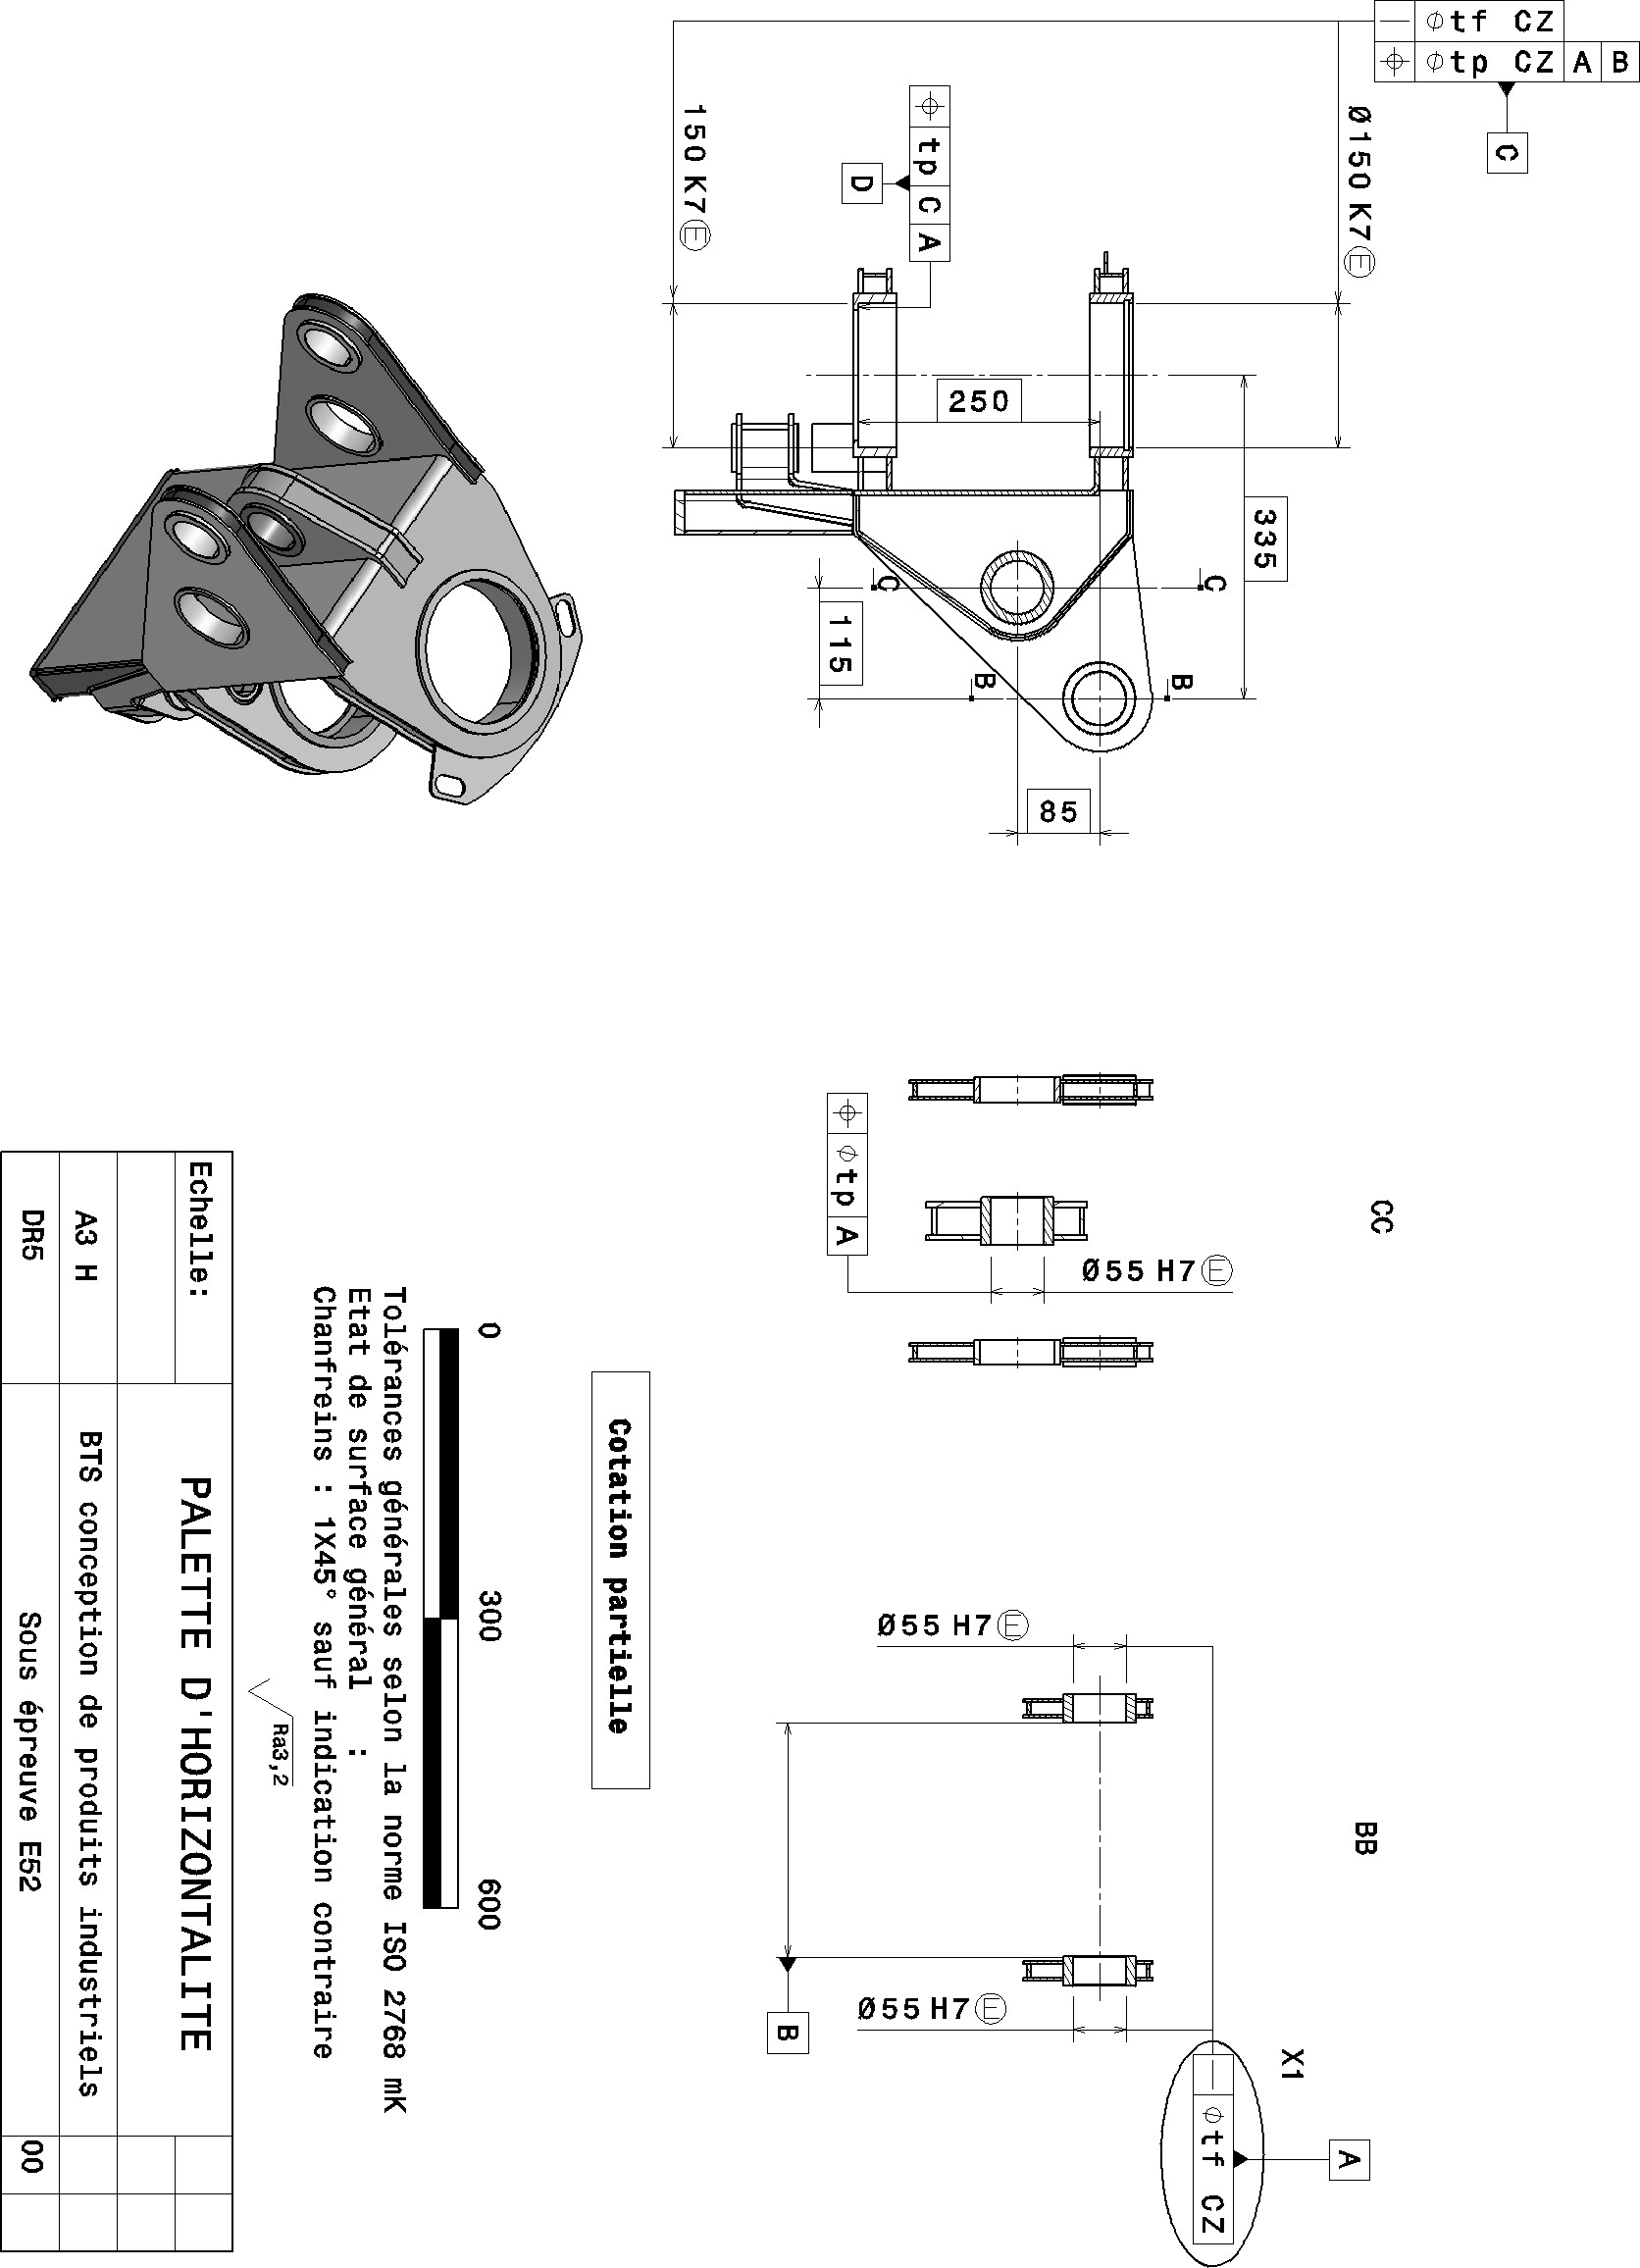
\includegraphics[width=\linewidth]{87_fig_03}}
%\end{center}

\begin{figure*}[!h]
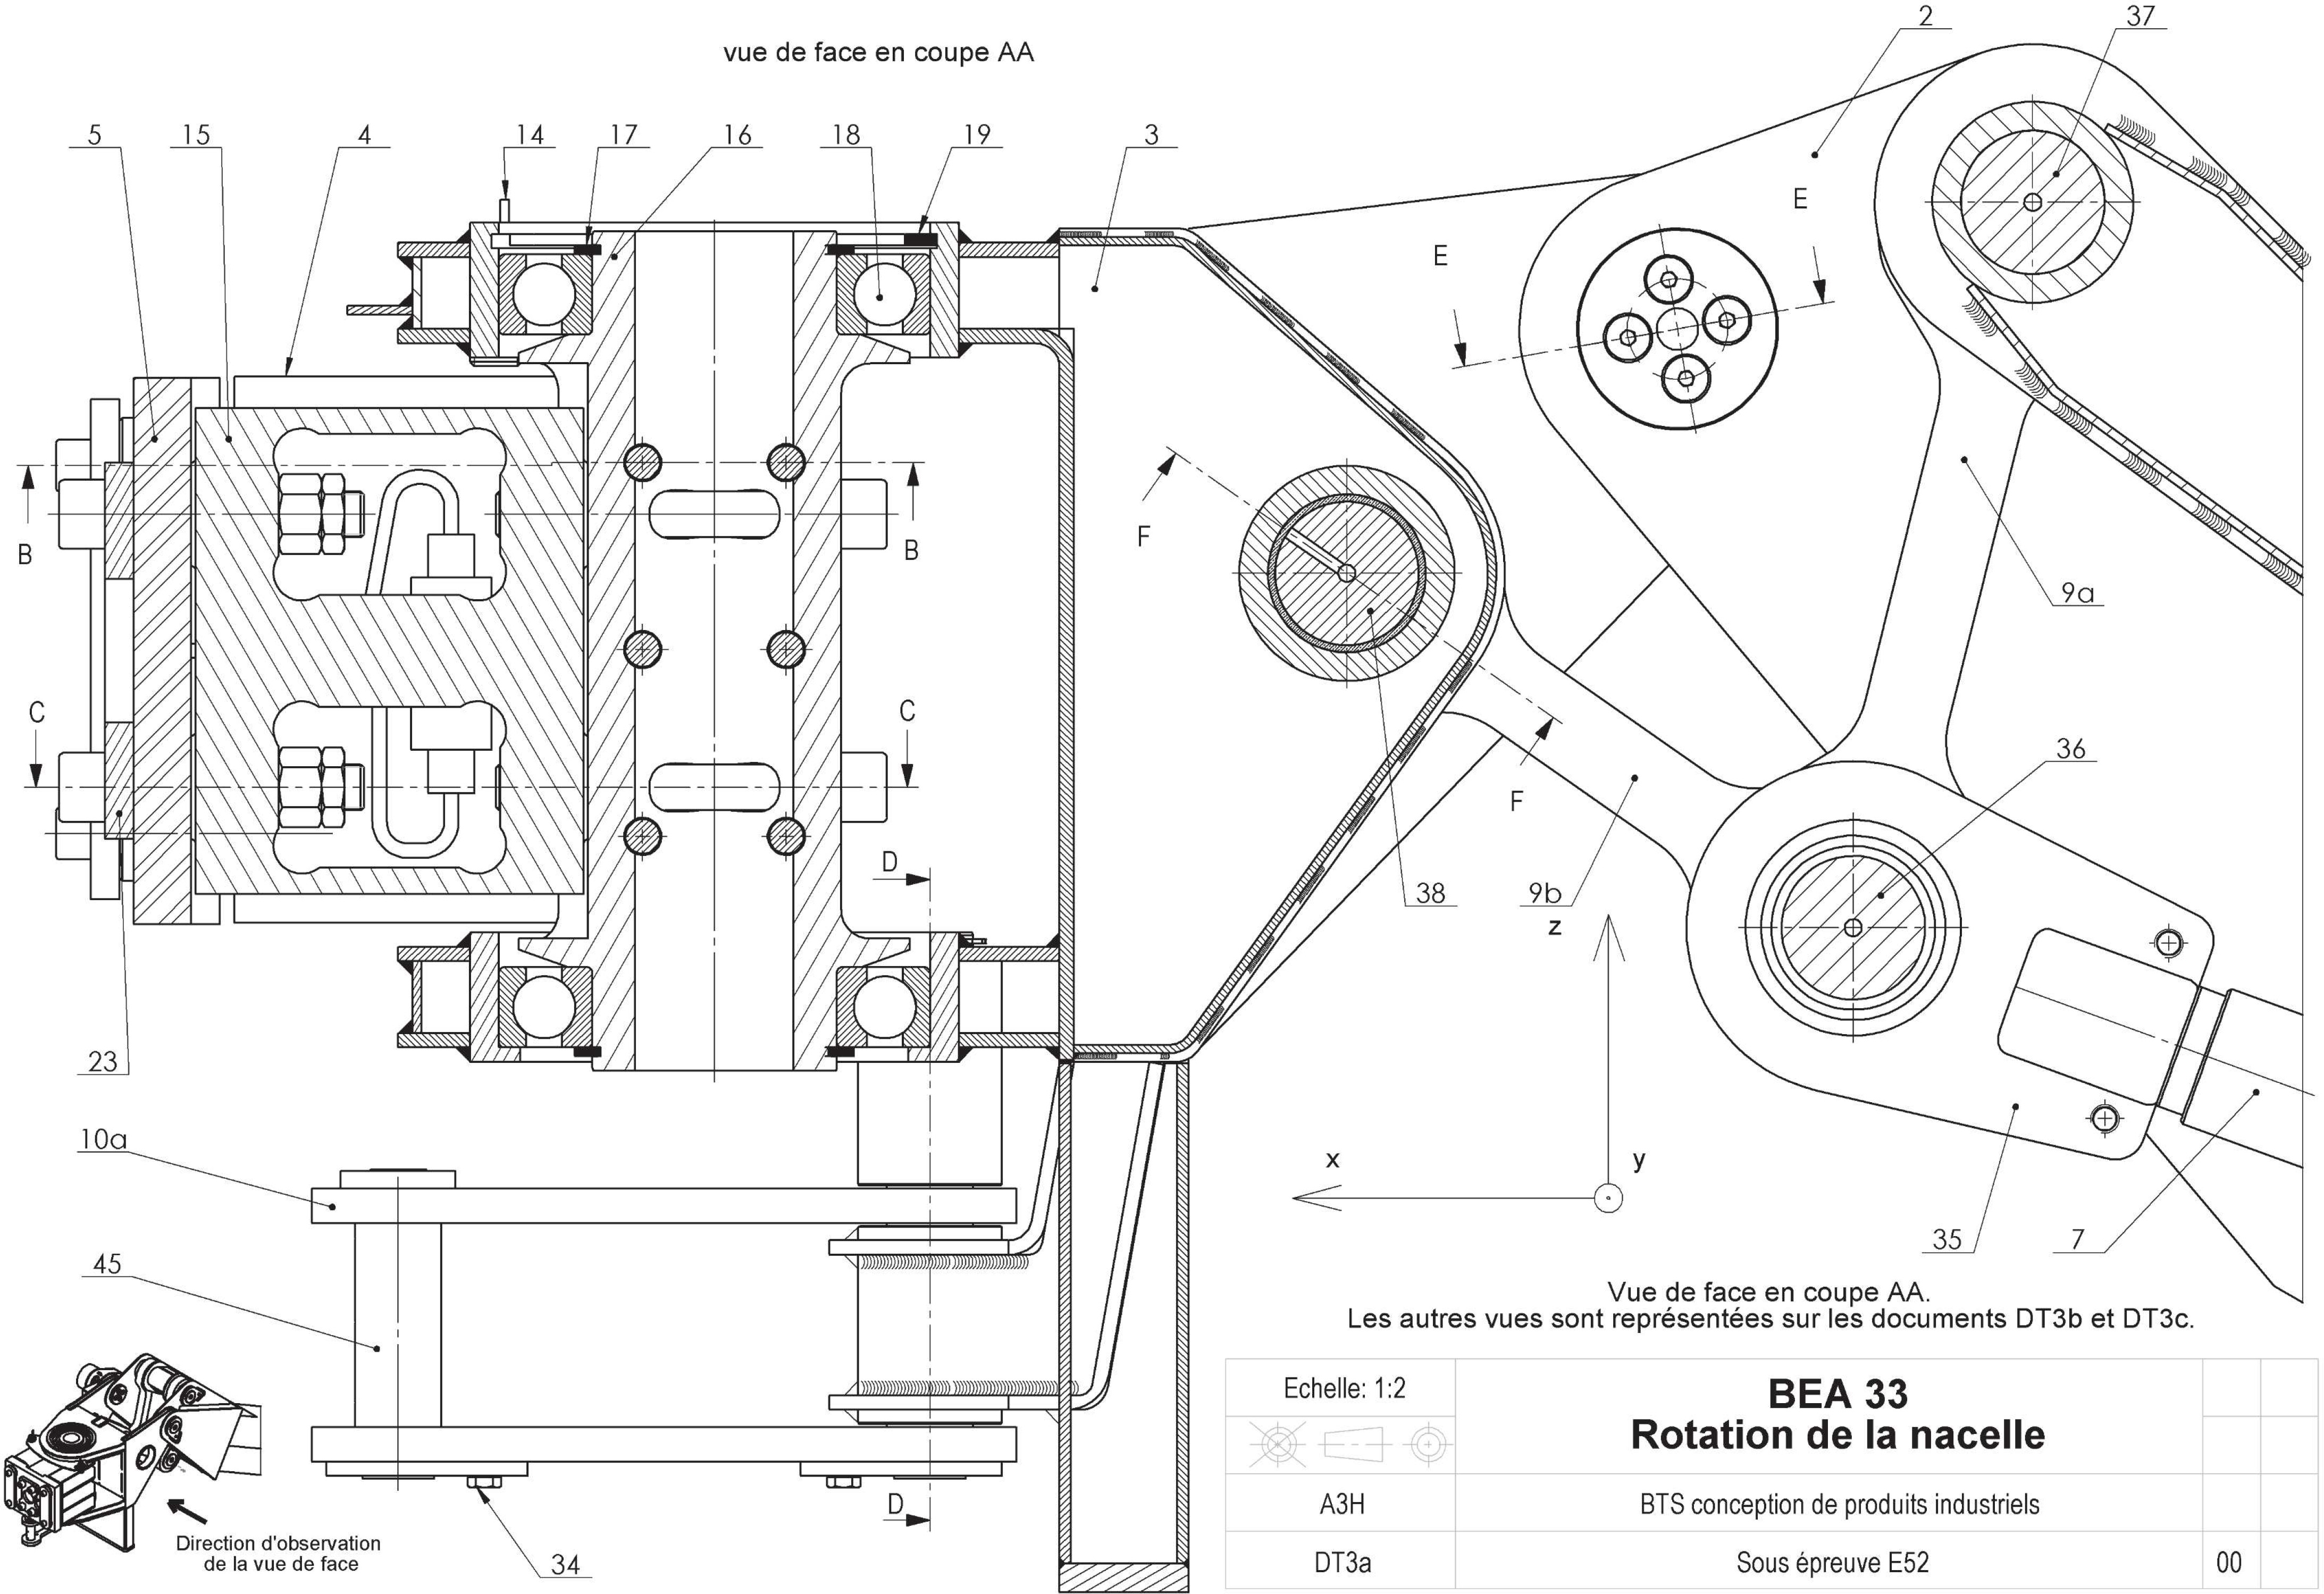
\includegraphics[height=\linewidth]{87_fig_04}
\end{figure*}

\begin{figure*}[!h]
{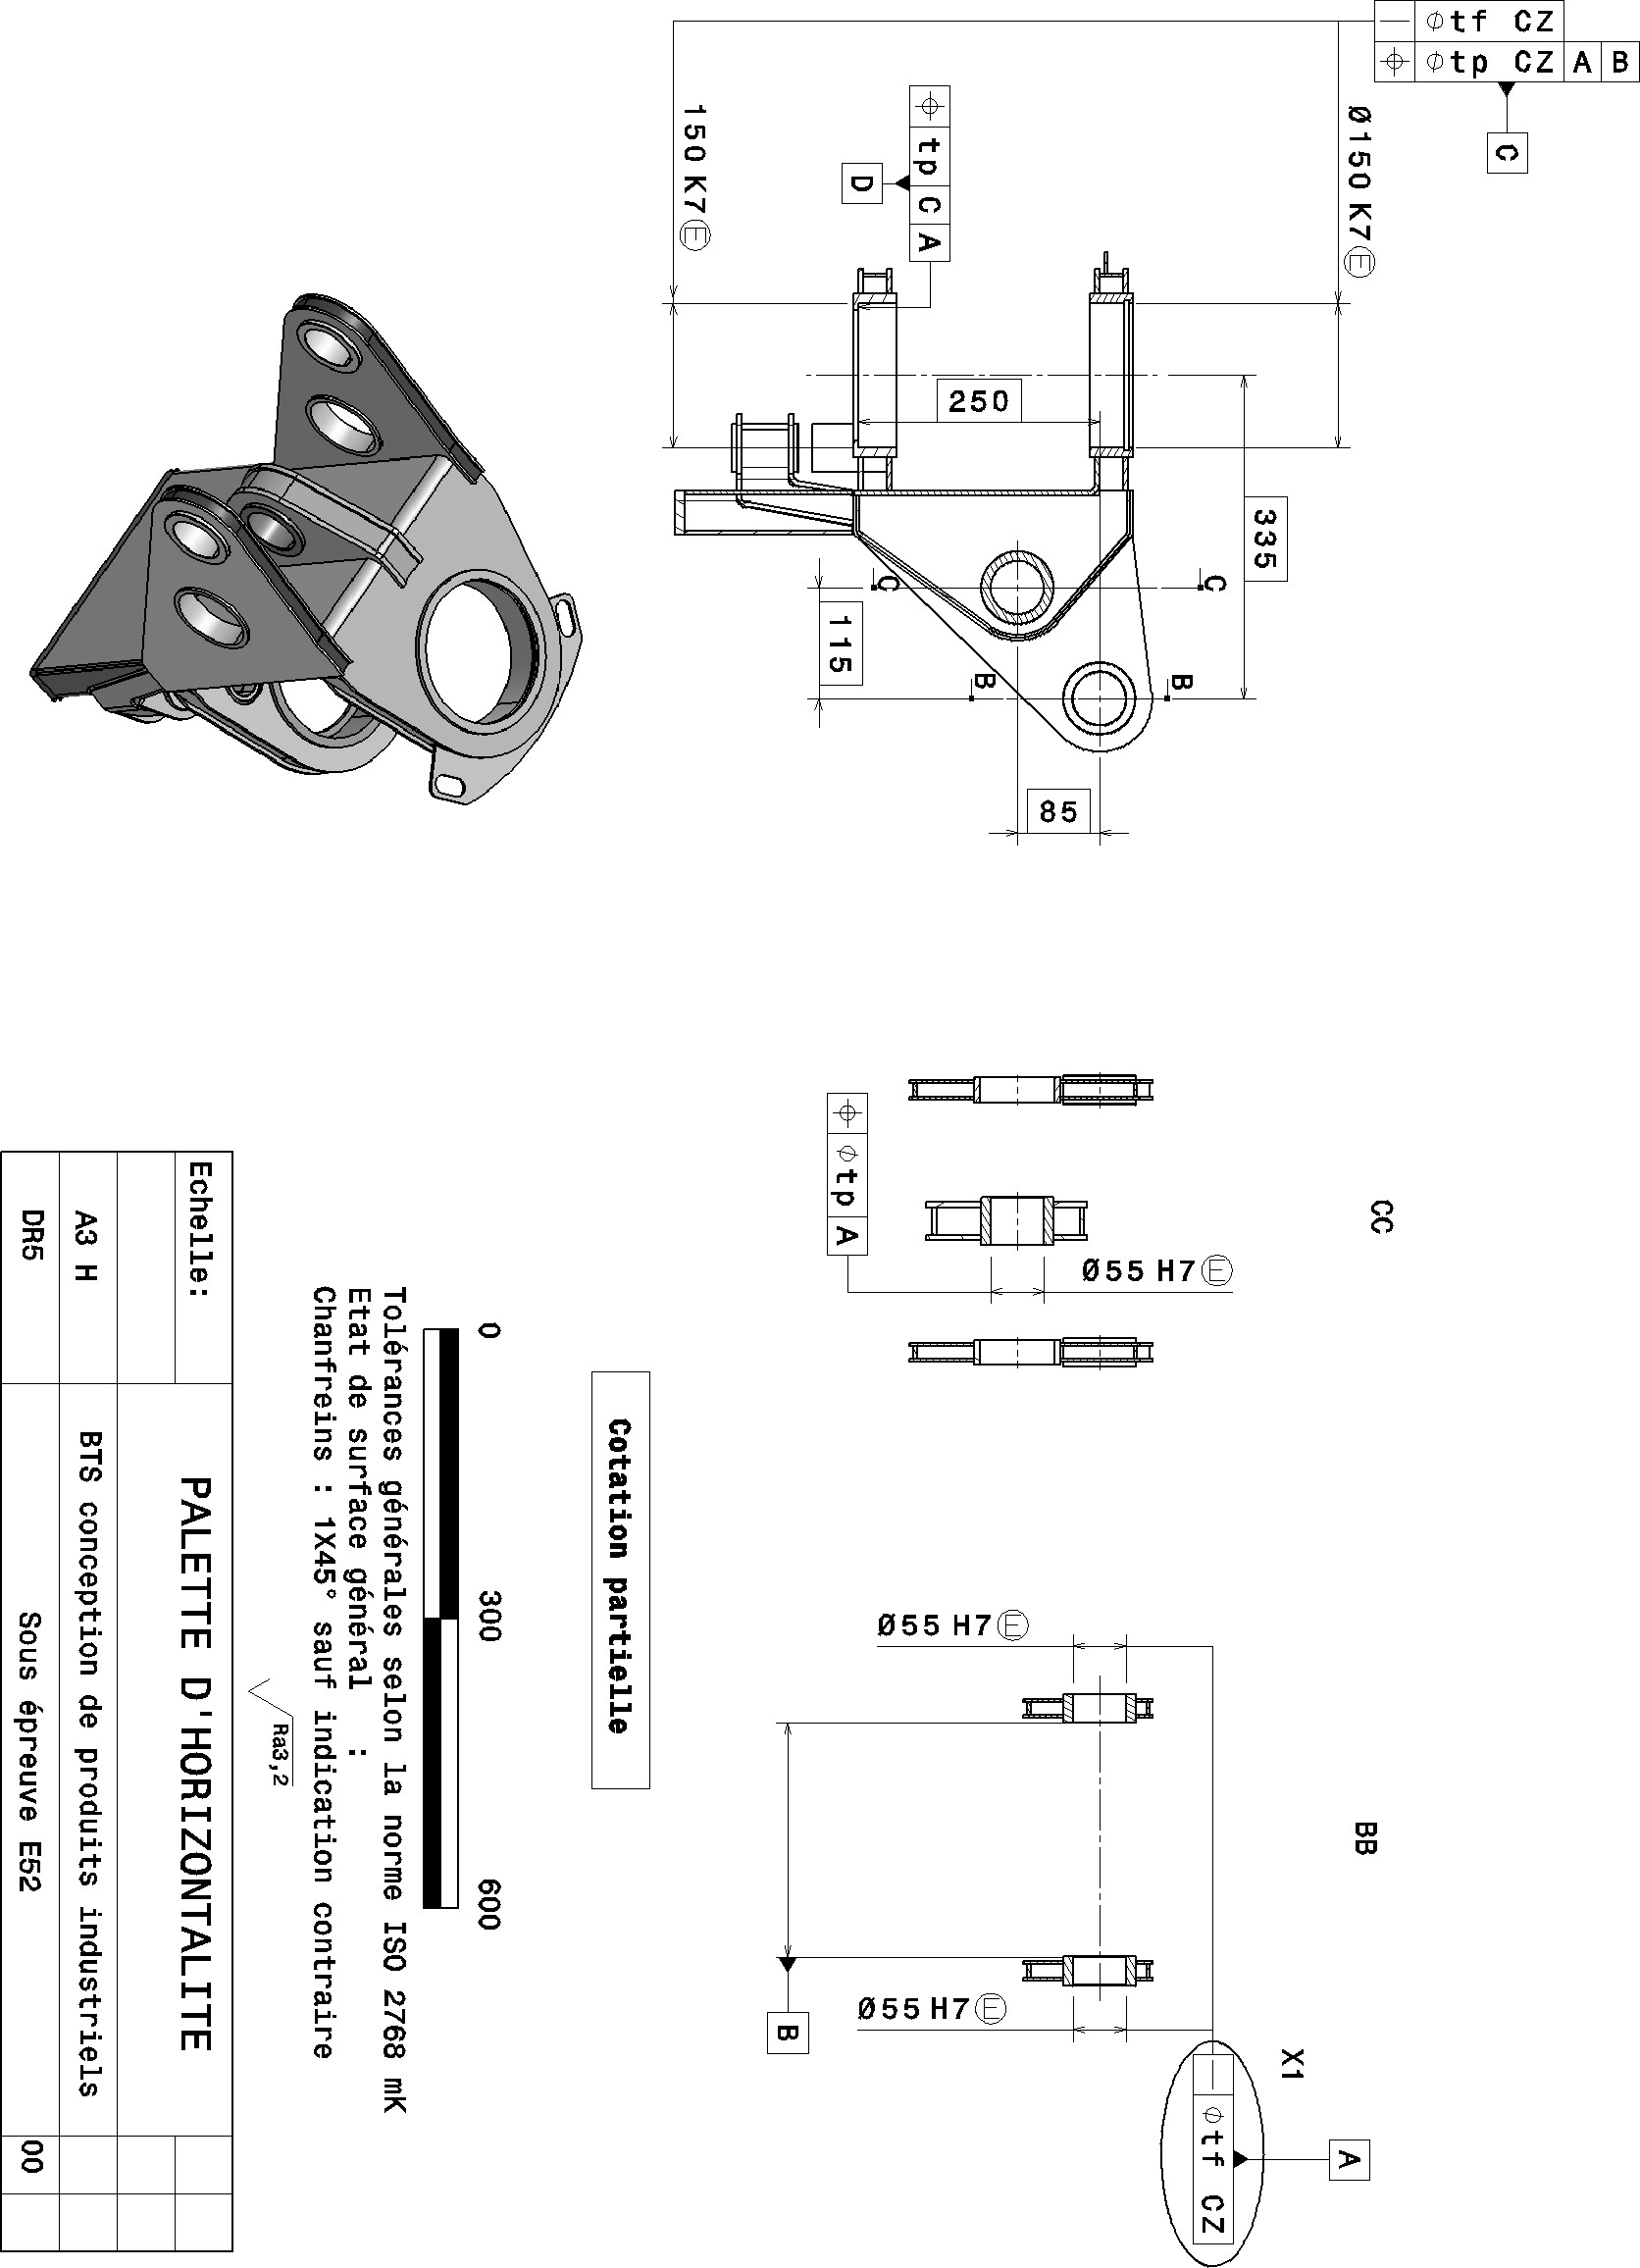
\includegraphics[width=.9\linewidth]{87_fig_03}}
\end{figure*}



\ifprof
\else
\begin{flushright}
\footnotesize{Corrigé  voir \ref{A5:05:87}.}
\end{flushright}%
\fi 